\chapter{會議記錄}
\section{5月23日會議紀錄}
討論事項: 討論機器人規格。首先繪製出各自的機器人。\\

\begin{figure}[hbt!]
\begin{center}
\label{523會議紀錄}
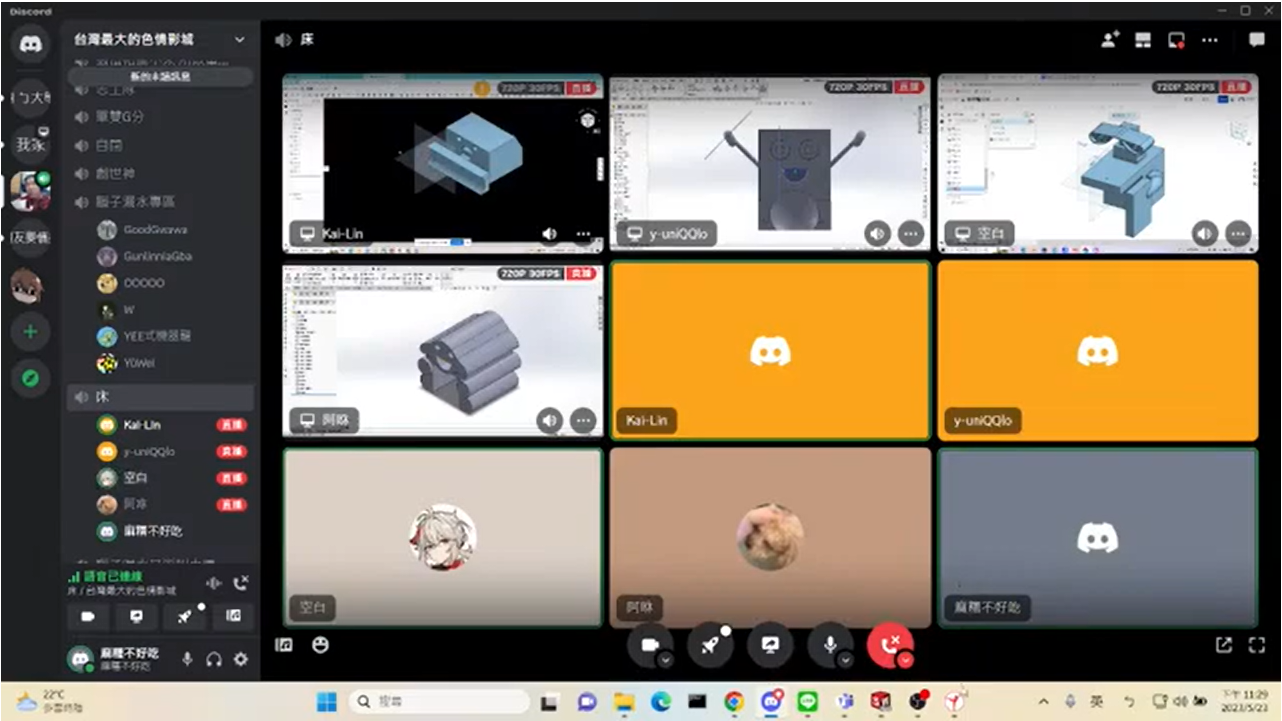
\includegraphics[width=12cm]{523開會紀錄}
\caption{\Large 523會議紀錄}
\end{center}
\end{figure}

\section{5月24日會議紀錄}
討論事項: 今日工作報告。\\

\begin{figure}[hbt!]
\begin{center}
\label{524會議紀錄}
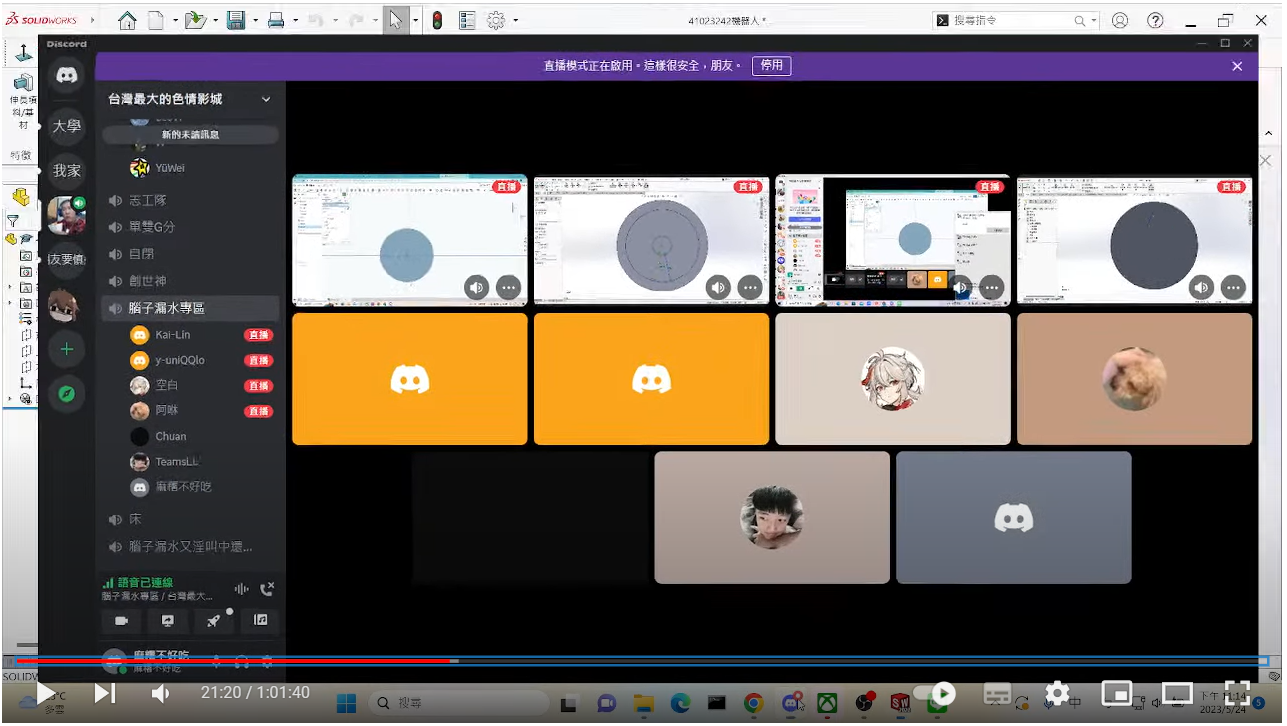
\includegraphics[width=10cm]{524會議紀錄}
\caption{\Large 524會議紀錄}
\end{center}
\end{figure}

41023242: 主持會議、上傳會議影片,組裝軸、把機器人匯入至CoppeliaSim嘗試動動看\

41023202: 繪製球員和球框場地\

41023212: 督導、協助\

41023229: 繪製計分裝置\

41023252: 督導、協助\

40923235: 繪製球員\

40923130: 程式修改\

40923115: 繪製球員\

40923235: 繪製球員\\

\section{5月31日會議紀錄}
討論事項: 把各自的機器人做修改並上傳,我們把場地跟球框重畫了,之前是場地球框分開畫,現在我們畫在一起這樣在協同的過程中比較方便進行,最後有讓我們的機器人裝上軸並試著走走看。\\

\begin{figure}[hbt!]
\begin{center}
\label{531會議紀錄}
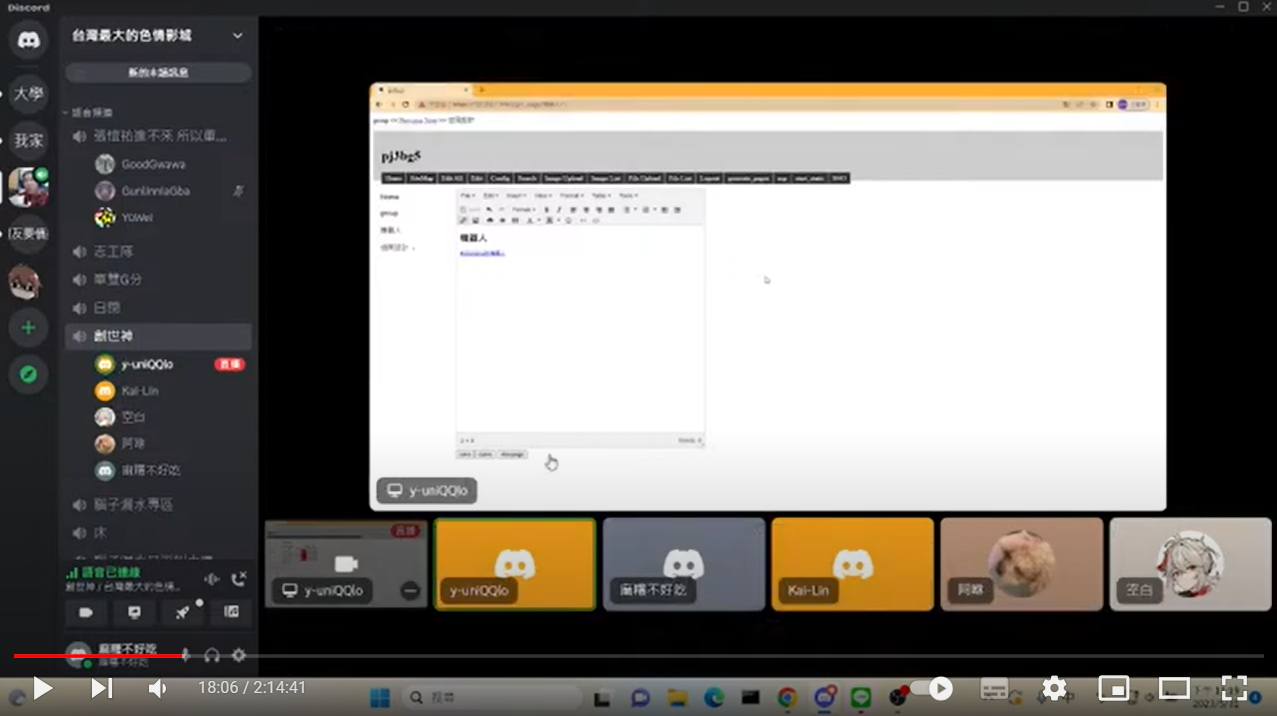
\includegraphics[width=12cm]{531會議紀錄}
\caption{\Large 531會議紀錄}
\end{center}
\end{figure}

\newpage
